%!TEX root = thesis.tex

\chapter{Soft, Unsupervised Classification with Spatio-Temporal Topic Models} \label{ch:topic-models-examples}
Our first two example applications explore the most direct connection to the existing topic modelling literature, performing unsupervised classification by defining a feature function, fitting a topic model, and grouping observations by their neighborhood's topic distribution. In Sec.~\ref{sec:substrate} we detail our work on deep-sea substrate classification from a challenging video dataset \citep{Kalmbach2016}. This application highlights the impressive closeness between the representation learned by our completely unsupervised technique and labels produced by a human expert which can be achieved by carefully designing a feature-function. Then in Sec.~\ref{sec:audio} we review our work on recognizing locations based on topic models of ambient audio \citep{Kalmbach2013}. This application highlights the suitability of spatio-temporal topic models for problems outside of computer vision, as well as the importance of spatio-temporal smoothness to representations learned in the absence of training targets.

\section{Substrate Classification from Repurposed Dive Videos} \label{sec:substrate}

\todo[inline]{Reduce the intro to this section?}\todo[inline]{I don't understand what you mean by "reduce", but this all ready pretty well to me as-is.}]
% \subsubsection{The need for soft substrate classifications from poor data}
% Paragraph: Why substrate classification matters
Substrate classification, the task of creating a spatial description of the nature of the seabed, is a fundamental factor in many aspects of ocean research.
Domain research in marine biology, physical oceanography and geology -- including classifying benthic \todo[inline]{say "(deep sea)" as well, this first time, for the CS person who doesn't recall what "benthic" means.} habitat, modelling deep-sea circulation and analyzing tectonic motion depends on accurate classification of substrate.

% Paragraph: Can't get enough hand labels
In the context of the deep sea, basic questions remain unanswered about what terrain can be found, particularly in geologically diverse mid-ocean ridge environments. High exploration cost and difficulty of sampling drive the need for remote sensing options for data acquisition, including visual and acoustic surveys, which in turn generate large volumes of data requiring analysis.
Manual analysis of substrate type is time consuming and requires geological expertise. Subjective factors, such as the choice of salient environmental features, make manual analysis for multidisciplinary use subject to observer bias.

% Paragraph: hard labels aren't really appropriate
Further, single-label classifications of substrate regions do not always adequately describe the complexity of types encoutered. In contrast, simple continuous valued substrate descriptors are sometimes used, such as the Udden-Wentworth Scale which proposes to describe the substrate by $-log_2(d)$ where d is average grain diameter in mm \citep{Krumbein1937}. Nevertheless, such descriptors are often impractical to evaluate with remote sensing, fail to capture the shape of the terrain, and do not account for the fact that terrain types, and therefore grain diameters, are rarely uniform within even a small region. Adding further dimensions to a substrate descriptor could account for some of these issues, at the cost of losing interpretability, and complicating the work of further domain research relying on this data. In this work we explore using soft classifications to add generality to the single-label paradigm, and seek to maintain interpretability by imposing a prior towards sparse label distributions. This approach can be seen as trying to maintain the best parts of both single label and higher dimensional substrate descriptors.

\begin{figure}
    \centering
    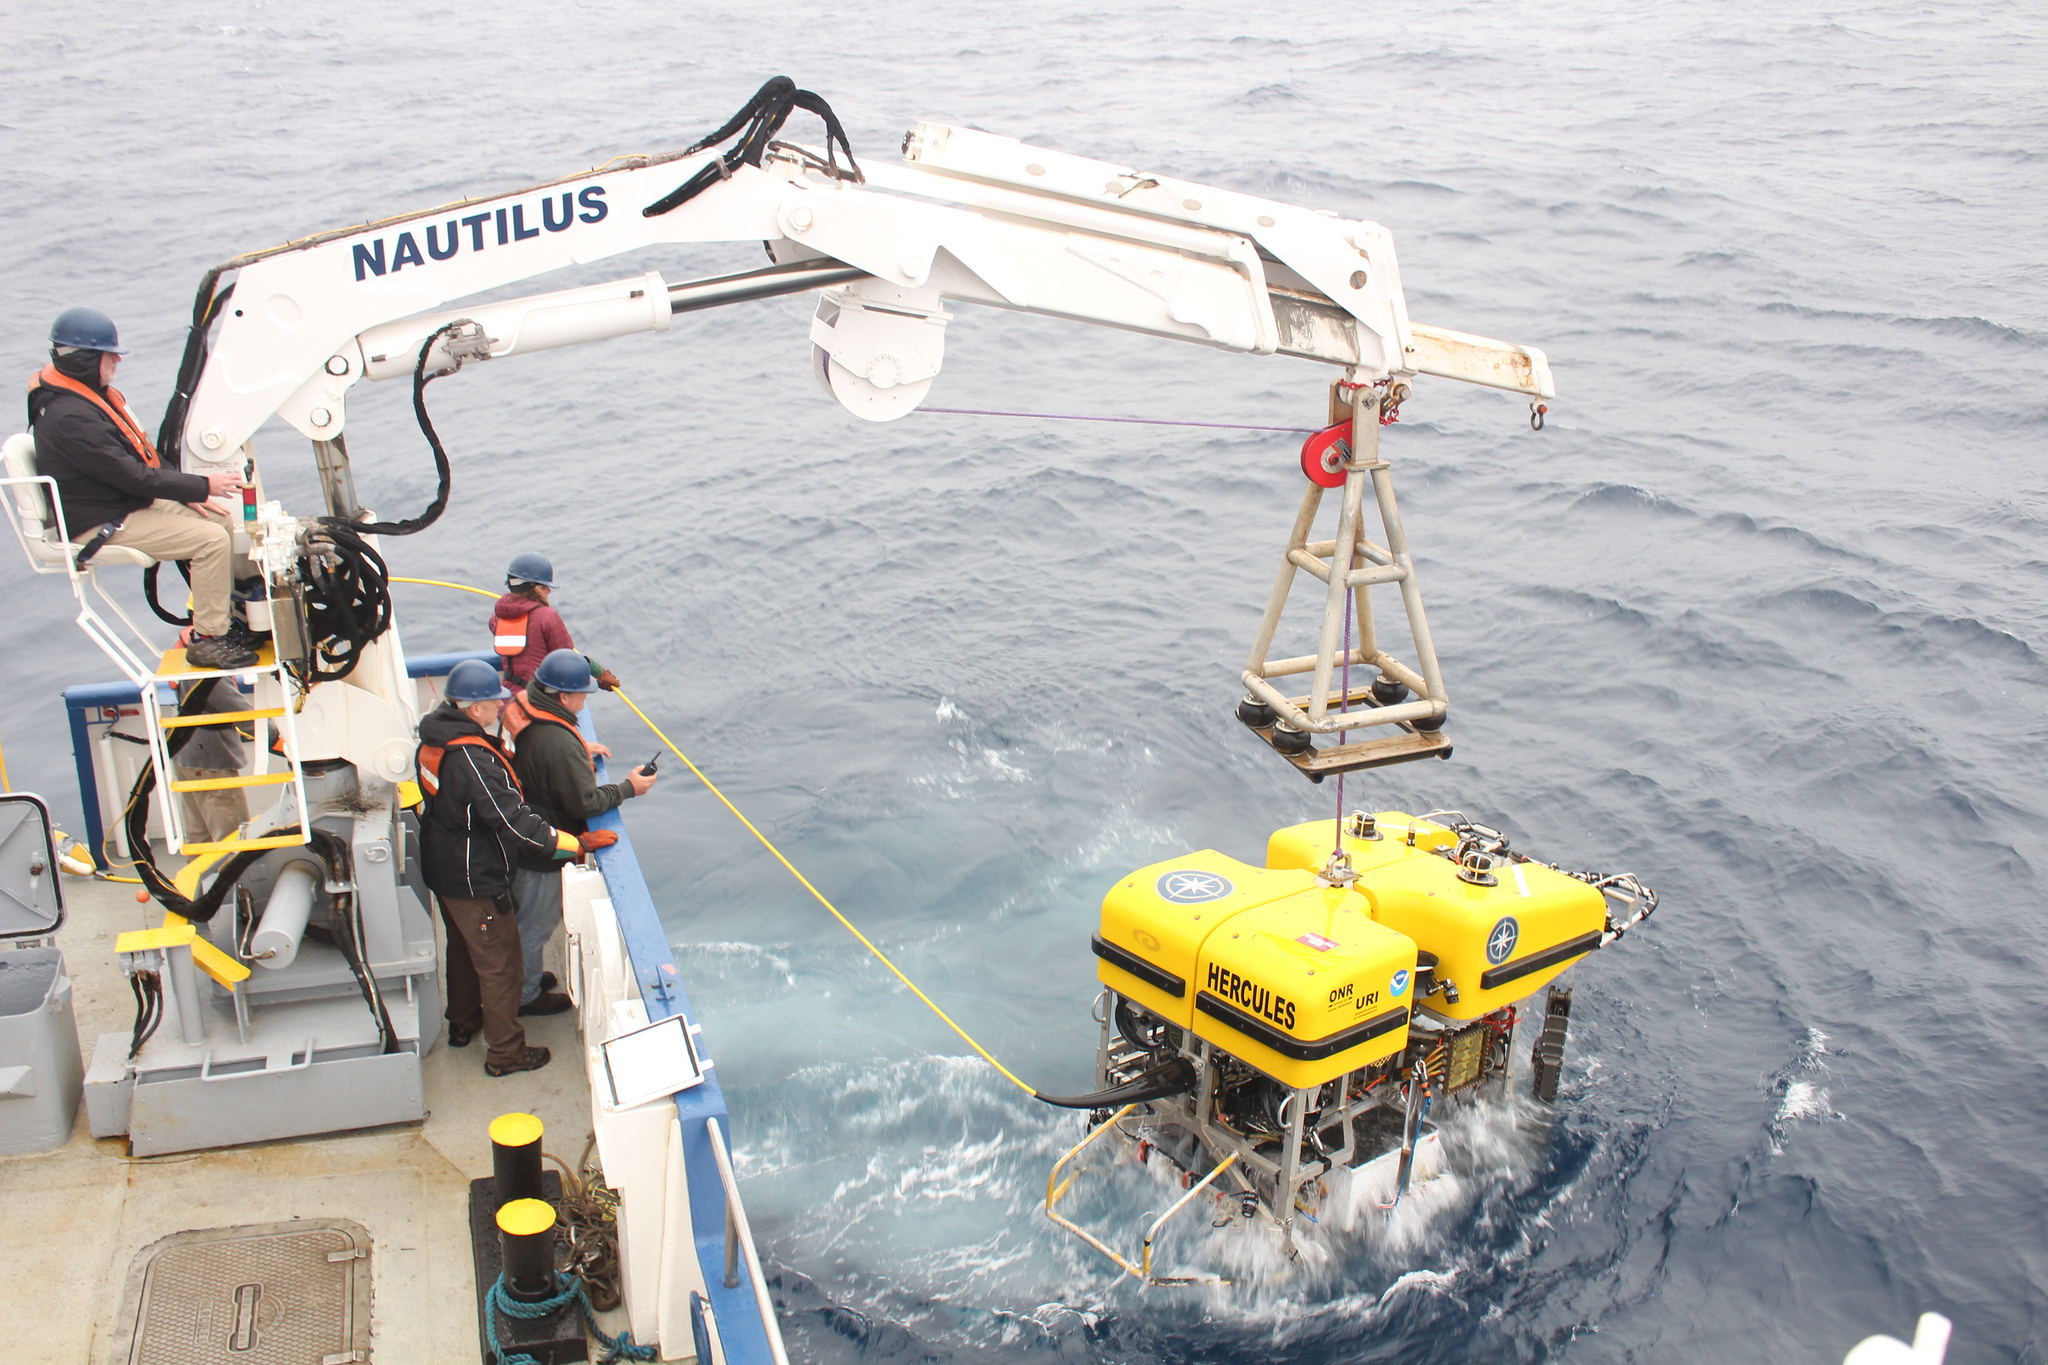
\includegraphics[width=0.65\textwidth]{figures/wacv/hercules}
    \caption{ROV Hercules returning to surface after a deep-sea cable route survey near Endeavour Ridge.}
    \label{fig:substrate-hercules}
\end{figure}
% 2-3 Paragraph: Can't just go get fresh data. Have to repurpose cable route surveys. Snow, lighting, and perspective.
Organizations such as Ocean Networks Canada (ONC), who operate cabled remote sub-sea observatories, regularly conduct manual visual cable route surveys in the deep-sea using Remotely Operated underwater Vehicles (ROVs). Collecting purpose-built deep-sea substrate measurements at high-spatial resolution is prohibitively expensive. In their absence, the historic video logs of these surveys contain extensive close-up video of the substrate, presenting the opportunity to train a substrate classification model.

Unfortunately, deep-sea ROV video contains significant artifacts due to a variety of factors. For instance hard, directional lighting is typical because sunlight does not reach the depths which interest us. Further, regions with the most interesting substrate such as hydro-geothermal regions, canyons, and seamounts all also feature challenging terrain for the ROV pilot. This leads to a wide variety of perspectives on the substrate. Finally, sediment and marine snow cloud the water column in the deep-sea, reducing contrast when the substrate is not very close to the camera, and filling images with particulate noise which confuses unmodified terrestrial computer vision techniques. Developing techniques to `see through' these artifacts to the substrate is necessary component of any system aiming to perform substrate classification using this data.

% Paragraph: ROST prior on classes is a reasonable assumption. So we just need to come up with a feature function that fits.
The spatio-temporal topic model's prior on neighborhood distributions is a good fit for this problem. It explicitly aims to capture the distribution of labels at each spatial location, rather than applying a single label like many techniques. Further, the sparse Dirichlet prior allows the modeller to ensure that the output distributions are more interpretable than a uniform or Gaussian prior when the meaning of the feature function is not well defined or understood with respect to the categories of interest. Finally, the smoothness component of the prior implemented by overlapping neighborhoods ensures that the topics reflect our intuition that labels at adjacent locations should be similar to one-another. By encouraging our model to capture our intuitions about the labels, we make the most of the large quantities of available unlabelled data so that with a highly restricted amount of labelled data we can learn to predict expert annotations.

\subsection{Using domain knowledge to define a feature function}

% 3 Paragraph: Feature extraction
As discussed in Ch.~\ref{sec:topic-models-inpractice}, one of the chief challenges of applying spatio-temporal topic models to a new domain is defining a feature function. In this work, we chose between standard, off the shelf, features combined with careful pre-processing steps to ensure that they encode the relevant information for substrate classification. Specifically we considered two feature functions: SIFT codebook and historgram of Improved Local Binary Patterns (ILBPs).

Based on the literature of topic models in computer vision, the most obvious choice of feature function is a codebook of Scale-Invariant Feature transform (SIFT) descriptors. SIFT is an extremely popular keypoint-based image feature, introduced by Lowe et. al as a scale and rotation invariant descriptor and detector for distinctive (i.e. easy to re-identify) points within an image \citep{Lowe2004}. SIFT has been remarkably successful in object recognition, image stitching, visual mapping, and many other computer vision tasks. We take SIFT as a reasonable surrogate for a variety of similar keypoint descriptors such as SURF and ORB. While SIFT features are 128-dimensional vectors, our topic models require discrete-valued features (words). Before running our algorithm, we produce a codebook of SIFT features. That is, using ROV logs from other dives, we compute the keypoints and descriptors for each frame. Then, choosing a vocabulary size (i.e. $V = 3000$), we compute the $V$ k-means centroids. At training time for our topic model we then extract keypoints for each new frame and compute the descriptors for each, replacing the descriptor with the index of the nearest neighbor centroid.

In contrast, Local Binary Patterns represent textures by encoding the local brightness variations in 9-pixel squares as 8-bit codes representing the relationship between each edge pixel and the center. Typically, these codes are computed for every pixel in an image, and grouped together into 256-bin histograms for non-overlapping windows. These histograms are then used as a descriptor for the textures in their windows. ILBP, originally introduced under the name MultiBlock LBP in \citep{Liao2007}, extends LBP, firstly by accommodating scaled pixel areas, and secondly by adding information about the center pixel. In ILBP, each pixel, including the center pixel, is compared to the mean value over an $N \times N$ pixel region. Liao et al. have shown that this improves the robustness of LBP as well as the ability to encode larger image structures. We use the multi-channel, multi-scale, windowed ILBP implementation described in \citep{Paris2012}. In contrast to descriptors such like SIFT, ILBPs are usually collected directly as histograms, and therefore no codebook is necessary. We concatenate the histograms for each window, scale, and color channel of an image, and treat each bin of the resulting histogram as a discrete feature when running our model.

% 2 Paragraph: Frame-rejection and resampling
In order to ensure that our model learns to distinguish substrate types, and not some other aspect of the dataset, it is important to carefully choose what data we will model.
A typical cable route survey creates 6-12 hours of continuous dive video, of which at least a few hours are usually irrelevant. For instance, surveys often contain extensive video of the ROV descending or ascending, sections with minutes to hours of video where the ROV is parked on the sea-floor, and yet more sections where the substrate is not in view due to challenging navitational conditions and sediments disturbed by the ROV itself.
Further, it is atypical for surveys to be conducted at constant speed, as the video is designed for live, manual analysis. To counter these effects, we first train a substrate detector, and then select a set of training images that are uniformly distributed in space.

We implement a substrate detector with a support vecor machine (SVM) on the spatial envelopes of relevant and irrelevant frames.
By spatial envelope, we refer to the holistic representation of the shape of a scene implemented as the GIST
descriptor described in \citep{oliva2001GIST}. GIST descriptors have been shown to encode high-level perceptual dimensions of the
spatial envelope such as ‘naturalness’, ‘openness’, ‘roughness’ etc. This descriptor is computed using a method based on Gabor filter responses in multiple orientations and scales, and in a grid of image windows across the image. GIST descriptors are appropriate as the local appearance of images with substrate varies dramatically, and the spatial envelope is more important that any local features.

We manually labelled 2000 randomly selected frames as either relevant or irrelevant (i.e. with or without substrate) for our subsequent classification problem. We trained an SVM using 1000 frames randomly selected from these 2000 labelled examples, and evaluated its performance on the other 1000. Table~\ref{tab:GIST-svm-performance} shows the precision and recall computed over all frames in the test set.

\begin{table}[t]
    \begin{center}
      \begin{tabular}{|c|cc|}
      \hline
         & Substrate & No Substrate \\
        \hline\hline
        Train Set (True)         & 564  & 436 \\
        Test Set (True)          & 589  & 411 \\
        Full Dataset (Estimated) & 6859 & 3141\\
        \hline
      \end{tabular}
      \caption{Numbers of relevant and irrelevant frames in our example video.}
      \label{tab:detection-statistics}
    \end{center}

    \begin{center}
      \begin{tabular}{|c|ccc|}
        \hline
         & Precision & Recall & F1-Score\\
        \hline\hline
        Train Set & 0.7942 & 0.9645 & 0.8711\\
        Test Set  & \textbf{0.8117} & \textbf{0.9440} & \textbf{0.8729}\\
        \hline
      \end{tabular}
      \caption{Performance of GIST SVM substrate detector.}
      \label{tab:GIST-svm-performance} 
    \end{center}
  \caption{GIST SVM performance}   
\end{table}

Dive logs contain navigation data collected by an ultra-short baseline (USBL) acoustic positioning device, in the form of Latitude, Longitude, and Depth measurements in addition to video. We converted Lat., Lon. into Eastings and Northings (meters East or North from start point), and time-synchronized the navigation and video logs. Next we ran our substrate detector on each frame from the video, discarding frames which did not contain substrate. Finally, we constructed a topic model training set by passing through the data in temporal order, and only keeping video frames which were more than a fixed radius away from all other points in the training set.

% 2 Paragraph: Image + feature filtering
In addition to ensuring that the training data comes only from potentially relevant locations, we must also ensure that the features encode the relevant aspects of the images.
Most images in the survey videos contain strong brightness variation at a low spatial frequency due to hard directional lighting and not the shape or texture of the substrate. Typical frames contain a well-lit foreground in the bottom middle and darker regions elsewhere. Due to marine snow and sediment, many images also contain particulate noise.
As perspective and other conditions change, these factors vary. To mitigate this,\todo[inline]{What is "this"}? we apply a 2D Gaussian bandpass filter with kernel
\todo[inline]{I suggest saying, to reduce the visual impact of the irrelevant, but ubiquitous, particular matter that is manifested as high-frequency image content, we use a bandpass filter"}
\begin{equation}
K = (1-e^{-(x^2+y^2)/2f_{low}^2}) \times e^{-(x^2+y^2)/2f_{high}^2}
\end{equation} 
where we set the frequency cutoff parameters $f_{low}$ and $f_{high}$ to be 4 and 100 cycles/image respectively based on the approximate minimum and maximum size of relevant substrate features. While particulate noise was a low spatial frequency detrimental factor, we found that the SIFT keypoints lost by smoothing over image details were more detrimental. To compensate, before extracting SIFT features we applied the highpass Guassian filter only. Finally, even with these preprocessing steps, not all features contain enough variation to help distinguish frames, and therefore only contribute noise to the modelling process. The concatenation of all the LBP histograms for an image results in a 10,752 dimensional histogram. We found that keeping only the $V = 3000$ bins with highest variance greatly reduced inference time for our topic model while slightly improving classification performance.

\begin{figure}
\begin{center}

\subfloat[]{
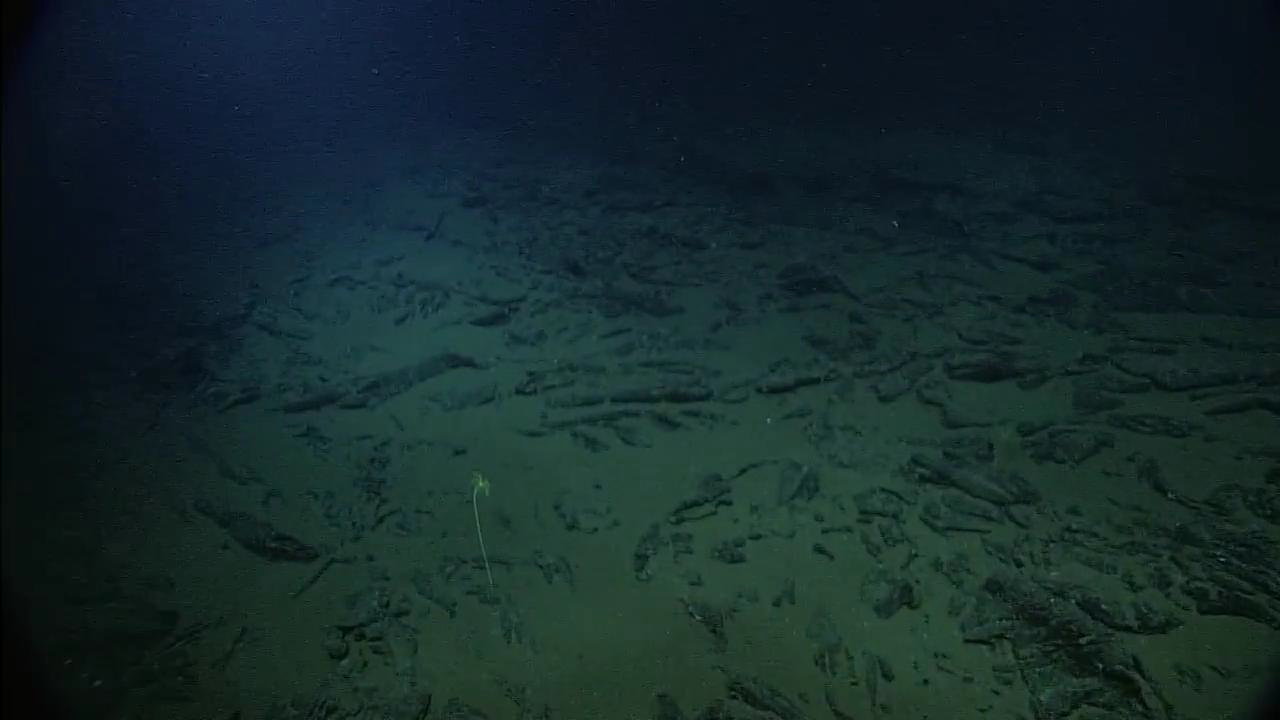
\includegraphics[width=0.48\columnwidth]{figures/wacv/r1218-beforefilter}
\label{fig:rov-eg-before}
}%
\subfloat[]{
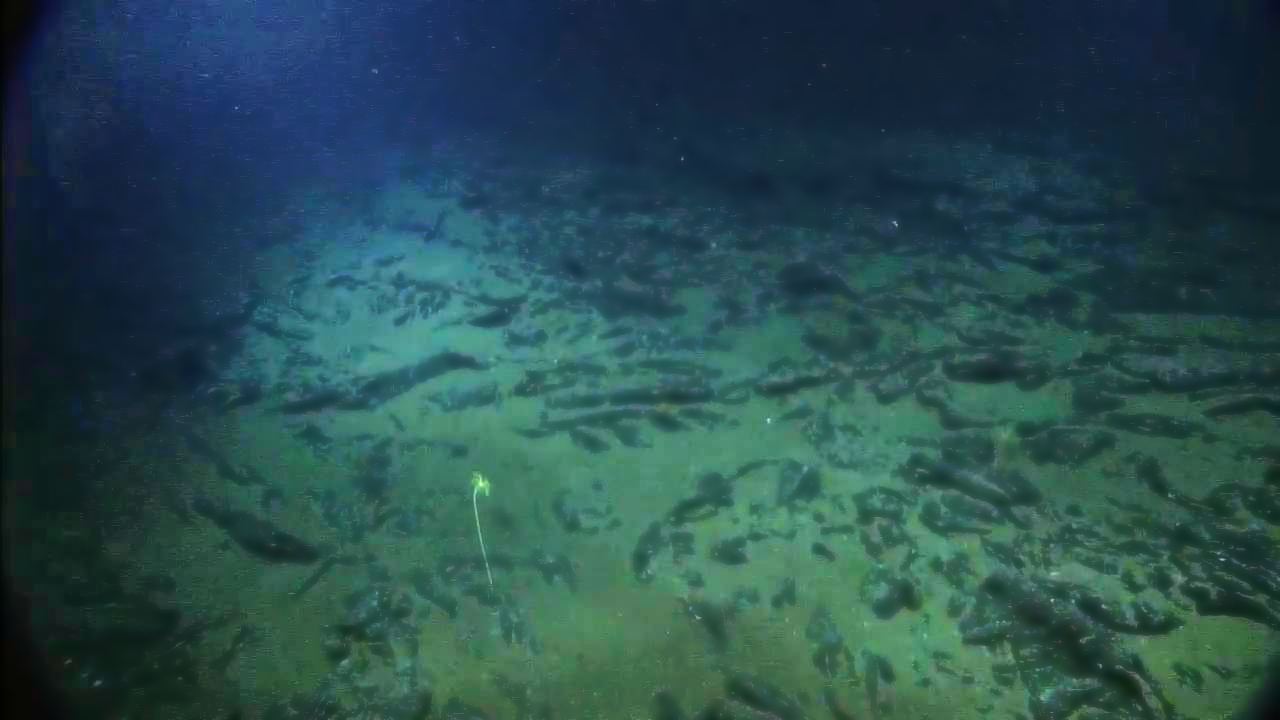
\includegraphics[width=0.48\columnwidth]{figures/wacv/r1218-afterfilter}
\label{fig:rov-eg-after}
}
\end{center}

\caption{
    \emph{Challenging ROV video data:}
	\protect\subref{fig:rov-eg-before} An example image collected by the ROV, before bandpass filtering and 
	\protect\subref{fig:rov-eg-after} after. 
}
\label{fig:rov-eg}
\end{figure}

\subsection{Evaluation}

% 2 Paragraph: Dataset description
We validate our method using data recorded at the Endeavour Segment of the Juan de Fuca Ridge, a midocean
ridge environment 300 km West of Vancouver Island, British Columbia, at approximately 2.2 km depth \citep{endeavourMPAPlan}. Specifically, our data is from the East Flank of Endeavour, a gently sloping area featuring a variety of substrate types. Mission objectives on this dive were to perform a visual survey for suitability of a scientific instrument installation -- much of the video shows substrate, but distance, angle, and speed are inconsistent throughout the recording.

The data consist of 30 fps HD video and 10 Hz USBL acoustic positioning. The ROV moved at an average rate of 0.5 knots (approx. 0.26 m/s), through two partially overlapping lawnmower patterns, one up and down a gentle slope, and one across the flat area at the base of the slope, with a total distance travelled of just over 5.6 km. We ran the substrate detector on every third frame (synchronized with the USBL data), and applied spatial subsampling with a minimum inter-frame distance of 1.5 m. This process resulted in a dataset of just over 3000 images.

Of these, we randomly selected 500 images, and with guidance from an expert in deep-sea geology, we defined seven categories that represent the types of substrate seen in the sample. These categories were ‘Sedimented’ (SED), ‘Interrupted Lava Flow’ (INT), Pillow Lava Flow’ (PIL), ‘Cliff or Wall’ (CLIFF), ‘Other Rock’ (O.RCK), ‘Turbid Water’ (TURB), and ‘Substrate out of Range’ (DARK). We labelled each image in this sample with proportions of these seven types, using a minimum increment of 0.25 for each category. Images exemplifying each category can be seen in Fig.~\ref{fig:substrate-best1gt}.

% 3 Paragraph: Pairing topics and classes
We generated the SIFT and LBP bag-of-words representations for each image in the full dataset, using the noise supression techniques described above. We used scale factor 2 for the ILBP region with a uniform 6x7 grid of non-overlapping windows. Initial experimentation showed that these values produced good results, and that additional scales did not cause significant improvement. We then fit the spatio-temporal topic model on each feature representation, choosing a neighborhood size of 15 m and 7 topics based on the estimated variation of the terrain and the number of true categories. We repeated this process for each pair of sparcity hyperparameters $\alpha, \beta \in \{0.01, 0.1, 0.2, 0.4, 0.8, 0.9, 0.99\}$. We chose the model with maximum log-probability on the held-out 500 image labelled set: $\alpha = 0.1, \beta = 0.1$ for SIFT and $\alpha = 0.1, \beta = 0.8$ for LBP. For these 500 datapoints, we infer topic assignments without updating the model. Although the most extreme values of $\alpha$ and $\beta$ tended to perform poorly, intermediate values had similar log-probabilities, and the exact hyperparameter choice did not seem to have a strong effect on the learned topics.

To evaluate the degree to which each ground-truth category was represented by some topic generated by our algorithm, we produced a one-to-one pairing between categories and topics. First, we calculated the Pearson $\rho$ correlation between each ground-truth category and each topic produced by our algorithm, using all 500 of the ground-truth frames. Then, we defined the cost of associating category $i$ with topic $j$ as $Cost(i, j) = 1 - \rho_{i,j}$, and used the well known Kuhn-Munkres (`Hungarian') Algorithm \citep{KuhnHungarian}, to find a minimal total cost assignment. In other words, we paired categories and topics so as to maximize the sum of correlations in the set of pairings. As the pairing is between topics and classes (a $7\times7$ matching problem), the cost of this process is negligeable.

We also computed 7 k-means centers for each image based on the distribution of each feature; SIFT, LBP, and top-3000-dimensions LBP. Then, we computed the cluster labels for test images, and applied the same optimal pairing algorithm for each. The results of these approaches offer insight into how well a method which does not take spatial smoothness into account might perform.

% 2 Paragraph: Describe tables. Impressive performance considering tiny amount of training data.
Fig.~\ref{fig:substrate-exout} shows the most representative frames for each topic. These images show the 7 frames that have the highest proportion of each topic throughout the dataset. Note that some topics were much more prevalent than others, so
an image may be among the best examples of a particular topic in the dataset without that topic being the top label for
the image. For instance, many of the strongest examples of interrupted lava flows contain more sediment than interrupted
lava flow. Comparison with the examples in Fig.~\ref{fig:substrate-best1gt} suggests that the topics assigned
to sediment, turbid water, and substrate out of range accurately recover their categories, and that the
other assignments are somewhat less accurate.

Tab.~\ref{tab:substrate-performance-7} reports the correlations between topics (or cluster labels) and ground-truth labels in the optimal pairing. Note that the topic model obtained the highest correlation of any method for every category, improving the strength of association by a mean of $3.58$ times over the best k-means approach (strength of association is defined as the absolute value of correlation). Strong positive correlations (i.e. near 1) indicate a linear relationship between variables, in this case indicating that the proportion of an image composed of a certain label can be predicted by a linear function of the weight of a single topic much more confidently than from its k-means cluster assignment. Also note that the LBP topic model outperformed the SIFT topic model for all classes except pillow lava, while at the same time the LBP k-means models also outperformed the SIFT k-means model for all classes except pillow lava. This suggests that the performance of a simplistic k-means model may be a reasonable simplistic surrogate for the full topic model when choosing which feature function to use for a topic model.

Note that for the LBP topic model, p-values were $ \lll 0.001 $, whereas for the other approaches, p-values varied, sometimes taking significantly higher values.
These p-values represent a strong rejection of the hypothesis that the topics were not correlated with the categories for our method, and a weaker one for the baseline strategies.

\begin{figure}
    \begin{minipage}{0.285\linewidth}
        \subfloat[][]{
            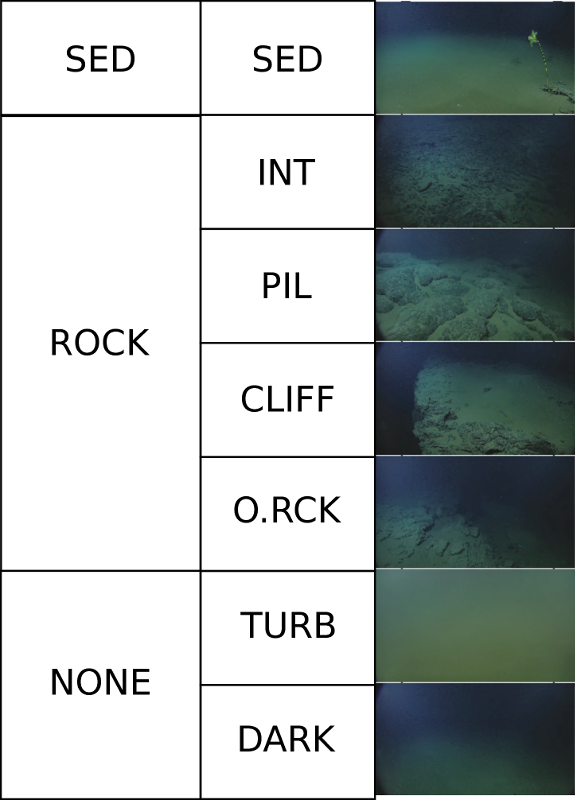
\includegraphics[width=0.979\textwidth]{figures/wacv/best1gt_table.png}
            \label{fig:substrate-best1gt}
        }
    \end{minipage}%
    \begin{minipage}{0.69\linewidth}
        \subfloat[][]{
            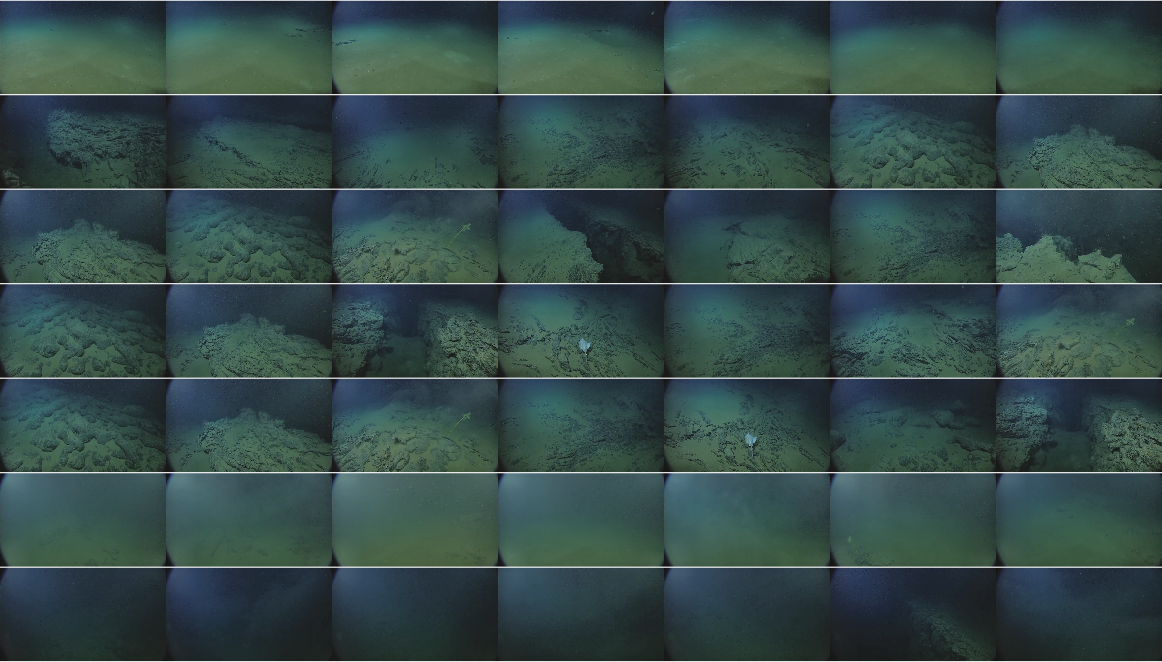
\includegraphics[width=0.98\textwidth]{figures/wacv/exout7.png}
            \label{fig:substrate-exout}
        }
    \end{minipage}
  \caption{
  	\emph{Example images of substrate types, and paired topics:}
    \protect\subref{fig:substrate-best1gt} Representative examples of the categories (top to bottom) `Sedimented', `Interrupted, 'Lava Flow'  `Pillow Lava Flow', `Cliff or Wall', `Other Rock', `Turbid Water', and `Substrate out of Range'.
	\protect\subref{fig:substrate-exout} Top 7 images paired with each category from
	\protect\subref{fig:substrate-best1gt}, based on the max-likelihood topic distribution, and the max-correlation pairing algorithm.
  }
  \label{fig:substrate-examples}
\end{figure}%

\begin{table}
    \centering
    \caption{\emph{Detailed substrate classification performance:}
    Pearson $\rho\left(498\right)$ for best-match topic with 7 ground truth categories (see \ref{fig:substrate-best1gt}). For ROST Filt. LBP p-value was $\ll 0.001$. Our method had the highest correlation for every category except PIL}
    \begin{tabular}{|c|ccccc|}
        \hline
              & K-M SIFT & K-M LBP & K-M Filt. LBP & ROST SIFT & \textbf{ROST Filt. LBP}\\
        \hline \hline
        SED   &  0.2898 &  0.3526 &  0.3661 & 0.5196 & \textbf{0.7489} \\
        INT   &  0.0718 &  0.0092 &  0.1116 & 0.3517 & \textbf{0.3899} \\
        PIL   &  0.4162 & -0.0029 &  0.0849 & \textbf{0.7024} & 0.3884 \\
        CLIFF &  0.1721 &  0.3474 &  0.2916 & 0.3601 & \textbf{0.4152} \\
        O.RCK & -0.0137 &  0.0508 & -0.0685 & 0.1901 & \textbf{0.2580} \\
        TURB  & -0.0271 &  0.6385 &  0.7509 & 0.1723 & \textbf{0.8153} \\
        DARK  &  0.3630 &  0.7509 &  0.3466 & 0.5454 & \textbf{0.5664} \\
        \hline
    \end{tabular}
    \label{tab:substrate-performance-7}

    \caption{\emph{High-level substrate classification performance:}
         Pearson $\rho\left(498\right)$ for best-match topic with 3 high-level categories. Our method had correlation coefficient above 0.7 for every category, with p-value $\ll 0.001$.}
    \begin{tabular}{|c|ccccc|}
        \hline
             & K-M SIFT & K-M LBP & K-M Filt. LBP & ROST SIFT & \textbf{ROST Filt. LBP}\\
        \hline \hline
        SED  &  0.4413 &  0.5059 &  0.5350 & 0.5196 & \textbf{0.7489} \\
        ROCK &  0.3492 &  0.3541 &  0.4930 & 0.6852 & \textbf{0.7156} \\
        NONE &  0.0459 &  0.4930 &  0.4601 & 0.3116 & \textbf{0.8015} \\
        \hline
    \end{tabular}
    \label{tab:substrate-performance-3}
    
\end{table}

In absolute terms, the values of the correlations reflect the intuition given by the best examples of each topic: The categories sediment, turbid water, and no substrate are each strongly correlated with their assigned topic, but the other categories are only weakly correlated with their assignment. Therefore, we additionally analyze our system's performance in classifying the high-level categories ‘Sediment’, ‘Rocky’, and ‘No Substrate’. These categories were constructed by combining the original categories, as seen in the leftmost column of Fig.~\ref{fig:substrate-examples}. We combined the groundtruth labels, topics, and labels for the three baseline methods by summing over the groups to be combined into each of the three categories. The performance of the resulting models is presented in Table~\ref{tab:substrate-performance-3}, showing that the LBP topics show strong predictive ability for the high-level class labels.

\begin{figure}
    \centering
    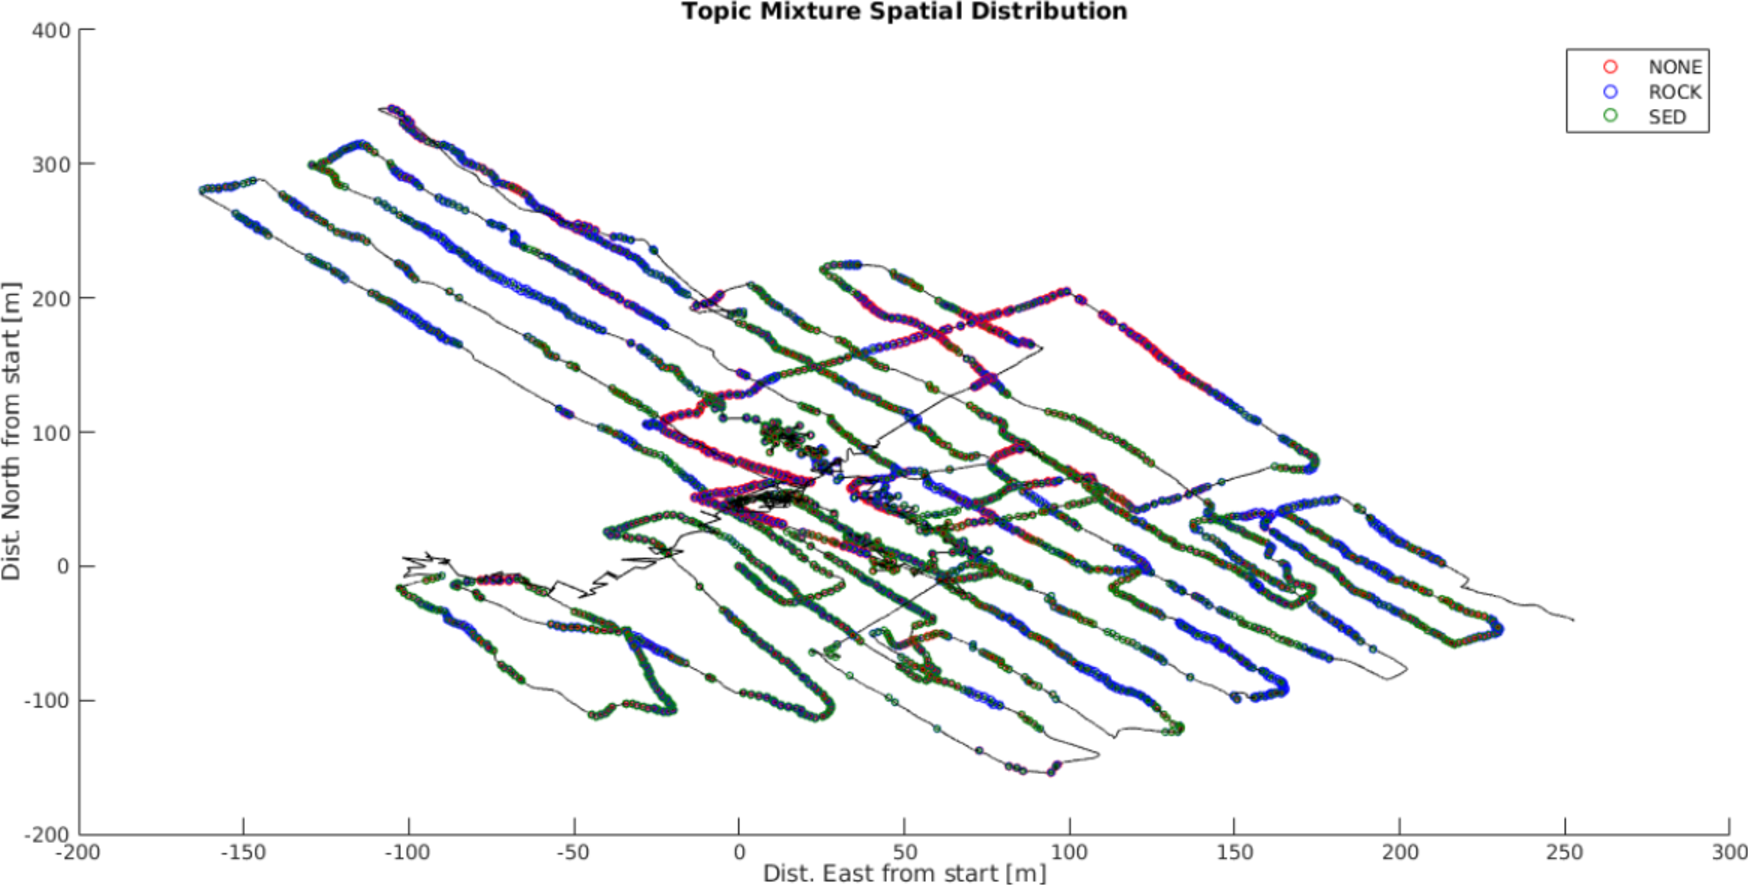
\includegraphics[width=0.9\textwidth]{figures/wacv/mixture-map2.pdf}
    \caption{\emph{Estimated substrate mixture map for Endeavour Ridge, BC:} ROV track with topic mixtures at each sample point. The line represents the path of the ROV, and each point is the location of a substrate sample image. At each point, there are circles for each of the three topics, with their sizes representing the mixture of the topics in that sample.}
    \label{fig:substrate-topic-map}
\end{figure}

Finally, in Fig.~\ref{fig:substrate-topic-map} we present the map of high-level substrate types produced by the LBP topic model. Maps of this type provide an interface between our method and biological or geological research which seeks to use information about substrate type. For instance, this map could be used in conjunction with a map of observations of a certain species to help answer questions about how habitat suitability is related to substrate type. Note that most points are described mainly by a single type, and that the substrate type assignments are spatially consistent. This outcome is crucial to an intuitive understanding of the map; it allows scientists to think naturally about regions of the substrate while still admitting that transitional areas which cannot be labelled as a single type exist. By choosing a spatial topic model to capture the visual data, we explicitly require our method to recover such an interpretable model. The automatic substrate classifications of our work are included in the GIS database for the Endeavour marine protected area, and are publicly available to researchers interested in the area \citep{Douglas2017} \footnote{An interactive version of this database is avilable online at \url{http://www.oceannetworks.ca/endeavour-hydrothermal-vents-marine-protected-area}}.

\section{Same-Place Recognition from Ambient Sound} \label{sec:audio}
%%% What happens when we try a very different feature function to text or bag-of-image-features? %%%
%%% How are semantic closeness, feature closeness, and topic closeness related? %%%
%%% 8 pg %%%

Our second example application of spatio-temporal topic models highlights the versatility of the model, operating on features from ambient audio. To the best of our knowledge, this is the first application of topic models to environmental audio that takes advantage of spatially coherent semantic regions. Our ability to consider temporal dependencies is crucial for this application as sound is fundamentally linked to temporal variation.

In this work we consider how to identify similar world regions by modelling the statistics of ambient sounds. We hypothesize that transitions in acoustic space correlate with transitions in other characteristic properties of the environment. Therefore, we aim to use the ambient sound to identify particular places and detect when we have returned to places we have already visited. In the context of robotics, we envision this system as one of many inputs to a filter-based probabilistic localization system. Common sensors such as range-finders and cameras often produce precise location hypotheses, but they are also susceptible to ambiguities which give rise to multi-modal beliefs. In contrast, an ambient-sound based localization system would give relatively imprecise hypotheses, only identifying the high-level region rather than an exact pose. However ambiguities in the soundscape of an environment are potentially very different from keypoint or corner ambiguities which confuse traditional sensing modalities. As a result, even such `weak' loop closures from sound could help improve the performance of localization systems.
\todo[inline]{Ambiguities... however ...}

Similar to the substrate classification example, in this work, an agent traverses the environment, makes observations along the way, and seeks to produce an intuitive description of these observations. As with substrate classification, an intuitive account is one that describes the world in terms of a few types, where neighboring locations should be assigned to the same type most of the time. Our spatio-temporal topic modelling framework aims to exploit this intuition to learn an appropriate representation without using any ground-truth labelling.

As we are interested in an input to a localization system, in this example the topic model features temporal smoothness rather than spatio-temporal, and observations are not accompanied by their position in the world. In addition, this system is designed to be fully unsupervised. That is, rather than matching topics with labels from a small training set, in this work we allow the topics to describe the data in whatever way represents it most accurately, and aim to extract information by comparing topic priors for different temporal neighborhoods to one-another directly.

\todo[inline]{Would be really nice to have a picture of the physical system (husky) and/or local region at ground level. Do you have either? Not critical, of course.} 

\subsection{Acoustic Features}
In the previous example we have seen the importance of carefully designing a feature function. For this example, we must take a short window of ambient audio and turn it into a discrete-valued feature. We extract such a feature using a k-means codebook of Mel Frequency Cepstral Coefficients (MFCC).

MFCCs are a compact representation of the timbre of an acoustic signal over a short time window. They have been commonly used to detect the source of a signal, especially in speaker and instrument recognition problems. Successive coefficients of a cepstrum represent the amount of the signal due to increasingly complex sinusoids. These are calculated using the inverse DFT of the log of squared DFT magnitude of a signal. MFCCs in particular use a re-weighting of the magnitude spectrum, so that lower frequencies are treated as more important than higher ones in order to achieve a more perceptually relevant cepstrum.

To be exact, MFCCs are computed using a filter bank with $L$ overlapping bands with triangular magnitude responses $\hat{h}_{l}[k]$ for $l=1, 2, ..., L$. The center frequency of band $l$ is given by $f_c(l) = 700 (e^{l/1127} - 1)$. The overlap percentage is constant and the centers are spaced further apart as frequency increases (see Fig.~\ref{fig:audio-melbank}), resulting in higher precision and weight on the lower frequency part of the signal. Given an input window $x$ the Mel-Frequency Cepstrum is given by
\begin{equation}
    cc(x) = \left| \mathcal{F}^{-1} \left( \log\left( \left|
    \sum_{l=0}^L
    \mathcal{F} \left(x\right) \hat{h}_l
    \right|^2 \right) \right) \right|^2
\end{equation}
The first $M$ coefficients can be computed efficiently using a DCT formulation where the filterbank is applied directly to the time-domain signal. In this domain, an interpretation where the $m$-th coefficient represents the part of the signal that can be described by the $m$-th cosine basis function arises.

\begin{figure}
    \centering
    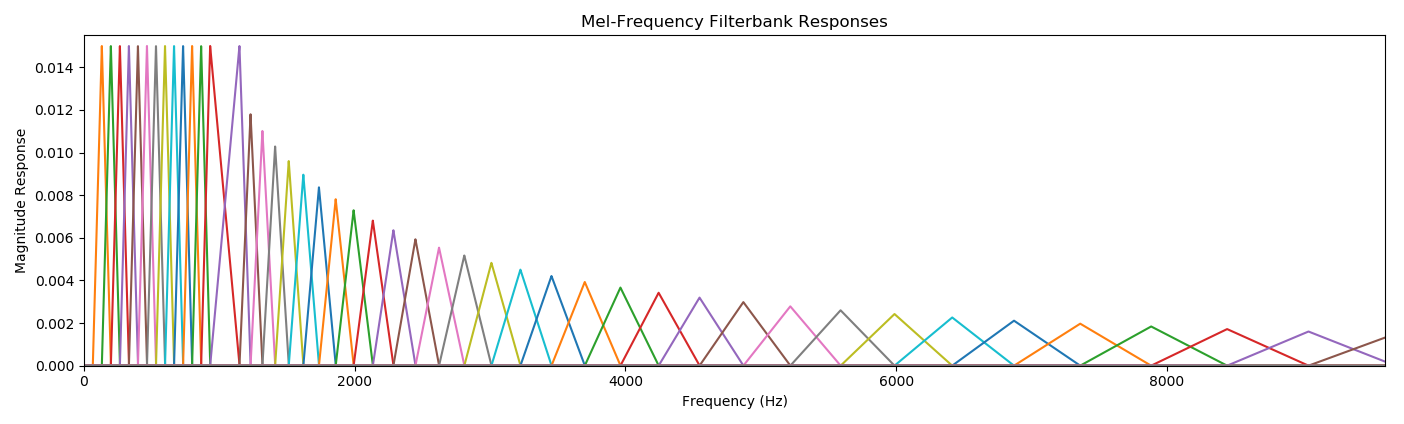
\includegraphics[width=\textwidth]{figures/audio/mel-responses.png}
    \caption{Mel- filterbank $h_l$ frequency responses for 48-bands and 50\% overlap. This filterbank implements perceptual reweighting of an audio signal.}
    \label{fig:audio-melbank}
\end{figure}

We consider the truncated cepstra, i.e. the first $M$ coefficients for short, overlapping windows of audio, as is typical for instrument and speaker identification problems which employ cepstral techniques. More detail on the construction of the filter bank and on choosing appropriate parameters for the window size and number of coefficients to calculate can be found in \citep{Sturm2010}.

\begin{figure}
    \centering
    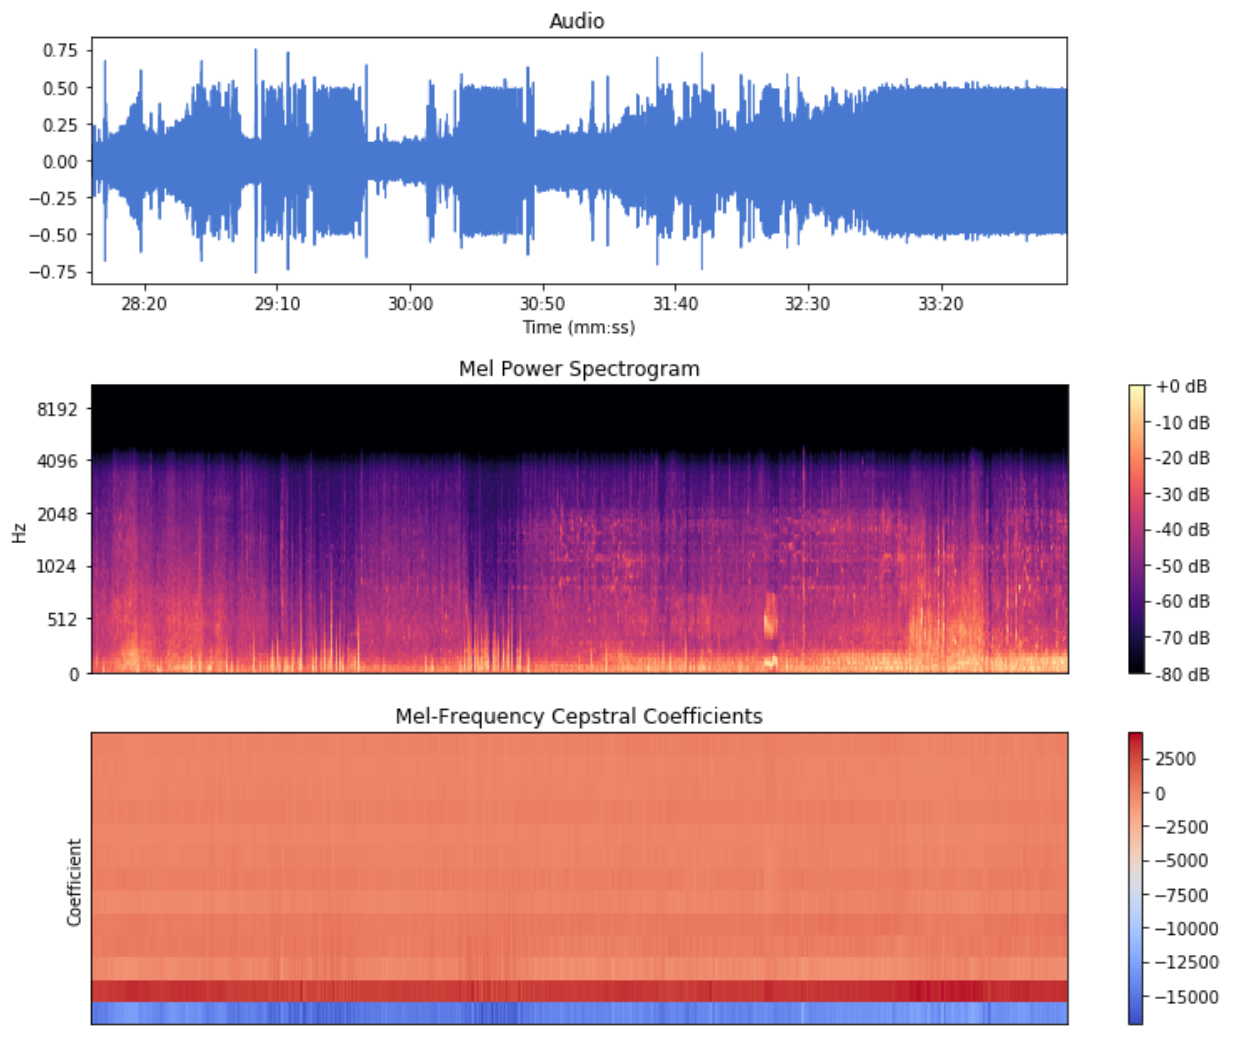
\includegraphics[width=\textwidth]{figures/audio/audio_processing.png}
    \caption{Segment of our audio processing pipeline corresponding to approximately 6 minutes from the `Campus' dataset detailed in \ref{fig:campus-map} (region labels 4,5,6,7). Compared to more traditional problems involving speech or music, obvious changes in the RMS amplitude and power spectrum are relatively subtle and infrequent.}
    \label{fig:audio-pipe}
\end{figure}

By only considering the first $M$ coefficients, we discard the most complex parts of the signal, and preserve only the `spectral envelope', i.e. the general shape of the sound. The higher order coefficients encode more ephemeral aspects of the sound, which in the case of matching ambiences would be detrimental to robustness.
Although the decomposition of an ambient sound's spectrum into envelope and noise (which coefficient is the appropriate boundary for a fundamentally noisy signal?) is much more obscure than that of an instrument or voice, we hypothesize that consistent noise sources such as air conditioners, passing vehicles, and distant vocal chatter are sufficiently distinct to be captured (for example, see Fig.~\ref{fig:audio-pipe}).  The final stage of our feature extractor is quantization via a k-means codebook, similar to the quantized SIFT features in the previous example. With reasonable window size and overlap parameters, this method produces dozens of feature observations per second.

\subsection{Evaluation}

We recorded audio datasets from two trajectories through the McGill campus and surrounding downtown area of Montreal, 51 and 43 minutes long respectively. The audio was recorded in stereo from a commodity hand-held video camera at a 44.1 kHZ sample rate while walking at approximately constant speed, and later combined into a single channel. The trajectories were chosen to contain varied sound environments, and contain both indoor and outdoor sounds, as well as sounds from busy and quiet environments. The maps of these trajectories are shown in Figs.~\ref{fig:campus-map} and~\ref{fig:figure8-map}. The dotted paths segments correspond to indoor environments. The \emph{Four-loops} dataset consists of four loops through the trajectory shown in the map, while \emph{Figure-8} is a trajectory which is topologically equivalent to figure `8', and is looped twice.  

We graphically represent when the trajectory returns to the same place with similarity matrices, where element $(i,j)$ is colored (non-black) if the agent was labelled to be in the same region at time $i$ and $j$, i.e., region labels $r_i = r_j$. For each trajectory, we hand-labelled the region for each temporal window according to the segments shown in Figs.~\ref{fig:campus-map} and~\ref{fig:figure8-map}, giving the similarity matrices seen in Fig.~\ref{fig:campus-groundtruth} and~\ref{fig:figure8-groundtruth}. Thus, colored blocks in the ground truth similarity matrices correspond to sets of locations that belong to a single spatial region with a consistent acoustic profile. For example, the red squares in Fig. \ref{fig:campus-groundtruth} correspond to sets of pairs of points along the trajectory that all have acoustic profiles produced at the roadway marked as region 1 in Fig. \ref{fig:campus-map}. 


\begin{figure}
    \begin{minipage}{0.45\textwidth}
        \subfloat[][]{
            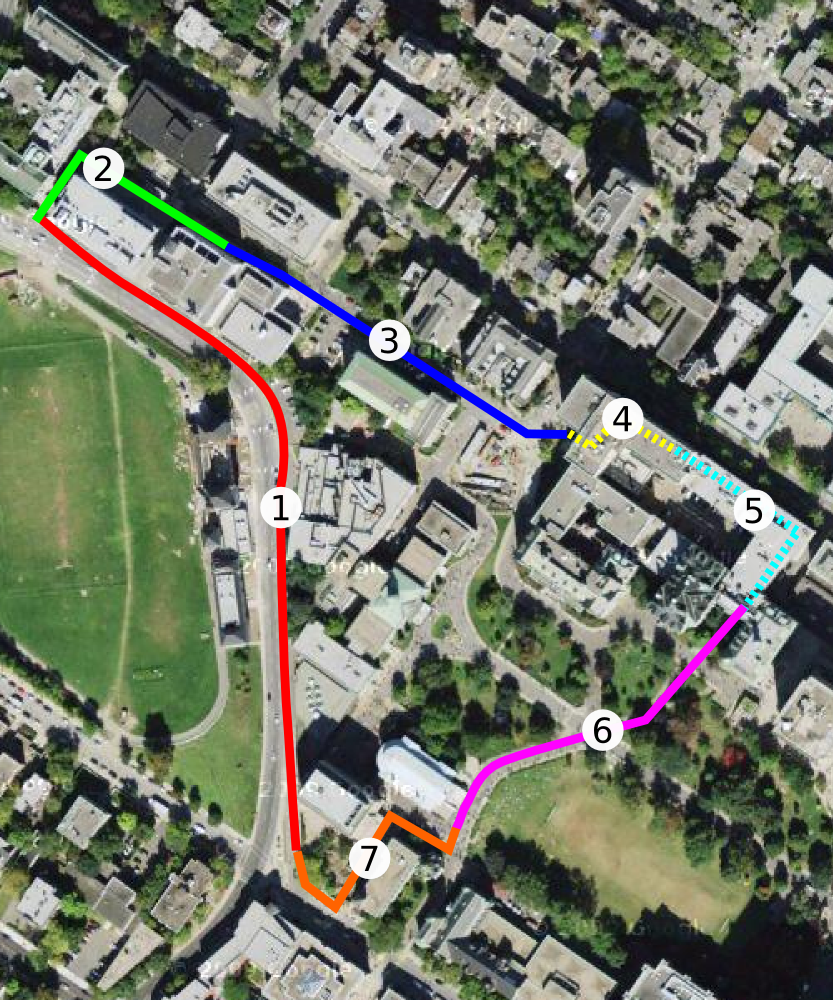
\includegraphics[width=\columnwidth]{figures/audio/campus/campus-map.png}
            \label{fig:campus-map}
        }
    \end{minipage} \hfill
    \begin{minipage}{0.48\textwidth}
        \subfloat[][]{
            
\includegraphics[width=0.45\columnwidth]{figures/audio/campus/groundtruth_color.pdf}
            \label{fig:campus-groundtruth}
        } %
        \subfloat[][]{
            
\includegraphics[width=0.45\columnwidth]{figures/audio/campus/dmat_words_campus+margin.pdf}
            \label{fig:campus-words}
        } \\
        \subfloat[][]{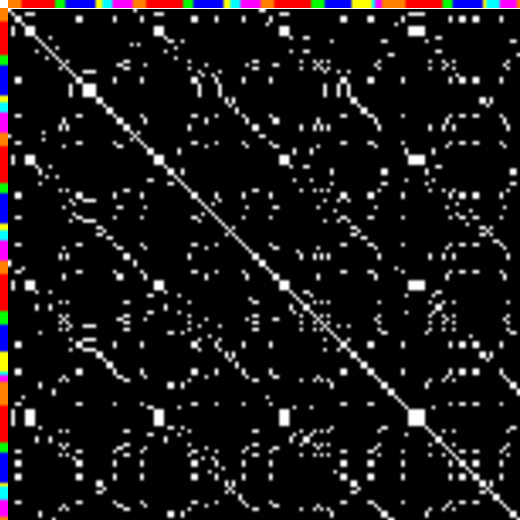
\includegraphics[width=0.455\columnwidth]{figures/audio/campus/dmat_regions_g0_campus+margin.pdf}
        \label{fig:campus-topicsg0}
        } %
        \subfloat[][]{
            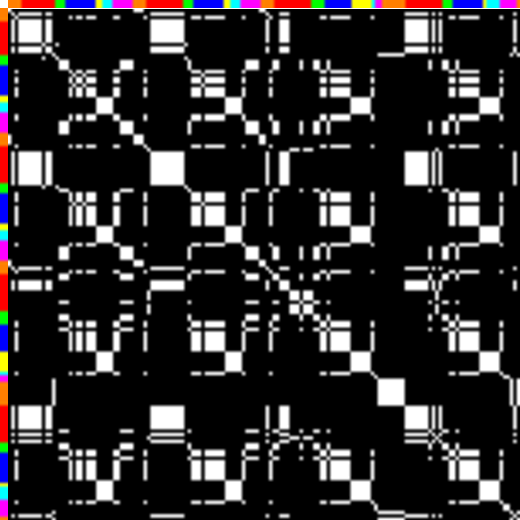
\includegraphics[width=0.455\columnwidth]{figures/audio/campus/dmat_regions_g4_campus+margin.pdf}
            \label{fig:campus-topicsg4}
        }%
    \end{minipage}
    
    \caption{\emph{Four-loops dataset:} 
        \protect\subref{fig:campus-map} Map showing the path traversed while recording the dataset.
        \protect\subref{fig:campus-groundtruth} Ground truth similarity matrix.
        \protect\subref{fig:campus-words} Similarity matrix for feature-based region labelling ($g=12$).
        \protect\subref{fig:campus-topicsg0} Similarity matrix for LDA-topics based region labelling ($g=0$).
        \protect\subref{fig:campus-topicsg4} Similarity matrix for temporally smoothed LDA region labelling ($g=4$).
    }
    \label{fig:dataset-campus}
\end{figure}

\begin{figure}
    \begin{minipage}{0.52\textwidth}
        \subfloat[][]{
            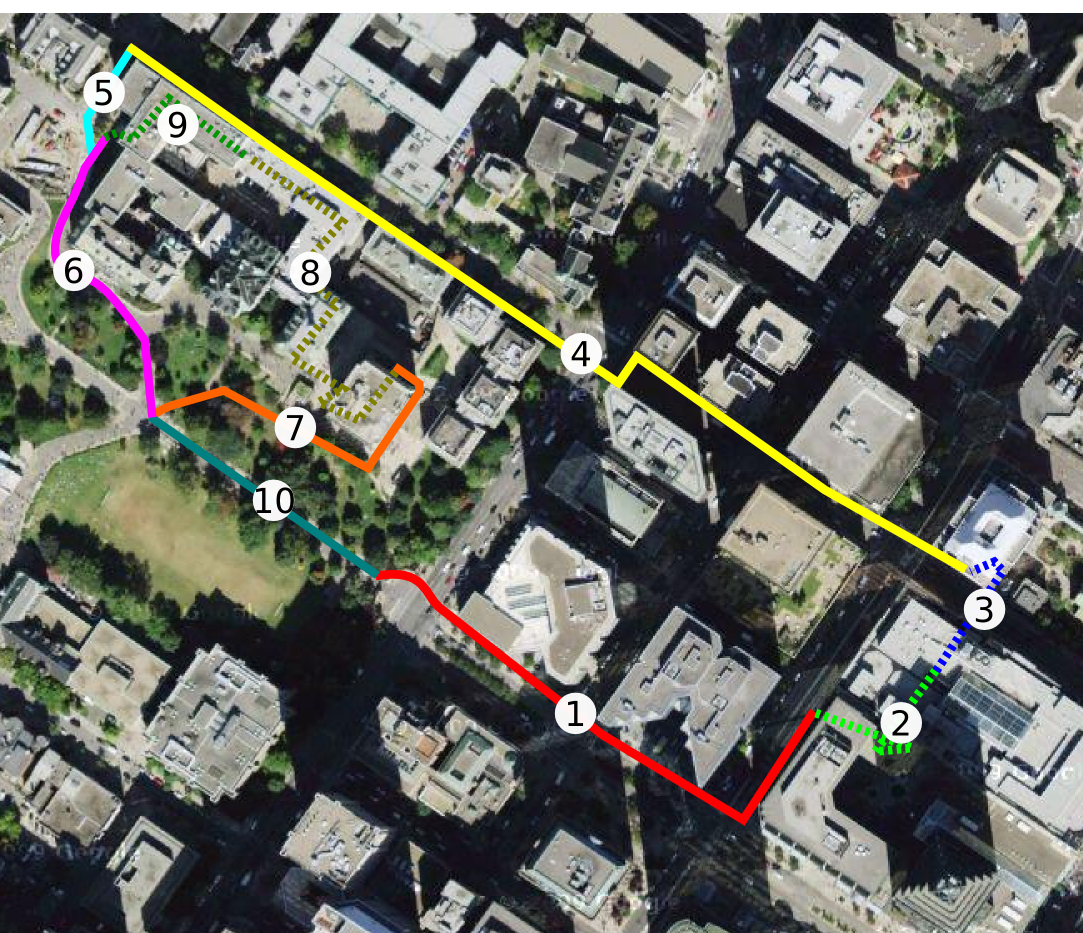
\includegraphics[width=\columnwidth]{figures/audio/figure8/figure8-map.png}
            \label{fig:figure8-map}
        }
    \end{minipage} \hfill
    \begin{minipage}{0.45\textwidth}
        \subfloat[][]{
            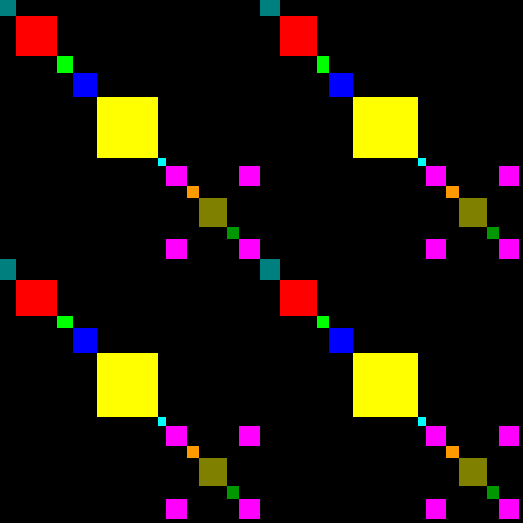
\includegraphics[width=0.46\columnwidth]{figures/audio/figure8/groundtruth_color.pdf}
            \label{fig:figure8-groundtruth}
        } %
        \subfloat[][]{
            
\includegraphics[width=0.46\columnwidth]{figures/audio/figure8/dmat_words_figure8+margin.pdf}
            \label{fig:figure8-words}
        } \\
        \subfloat[][]{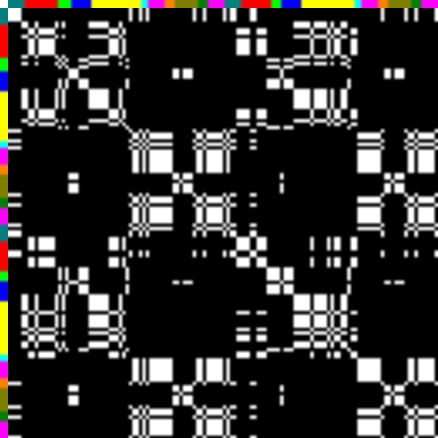
\includegraphics[width=0.46\columnwidth]{figures/audio/figure8/dmat_regions_g0_figure8+margin.pdf}
        \label{fig:figure8-topicsg0}
        } %
        \subfloat[][]{
            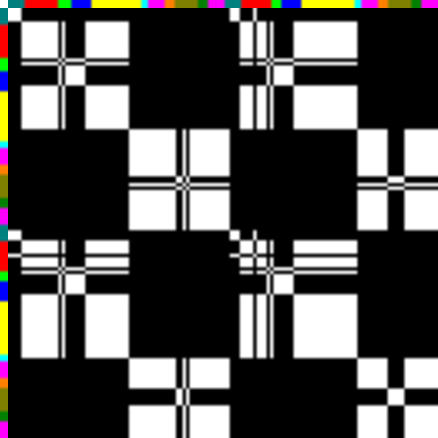
\includegraphics[width=0.46\columnwidth]{figures/audio/figure8/dmat_regions_g2_figure8+margin.pdf}
            \label{fig:figure8-topicsg2}
        }%
    \end{minipage}
    
    \caption{\emph{Figure-8 dataset:} 
        \protect\subref{fig:figure8-map} Map showing the path traversed while recording the dataset.
        \protect\subref{fig:figure8-groundtruth} Ground truth similarity matrix.
        \protect\subref{fig:figure8-words} Similarity matrix for feature-based region labelling ($g=14$).
        \protect\subref{fig:figure8-topicsg0} Similarity matrix for LDA-topics based region labelling ($g=0$).
        \protect\subref{fig:figure8-topicsg2} Similarity matrix for temporally smoothed LDA region labelling ($g=2$).
    }
    \label{fig:dataset-f8}
\end{figure}

The regions were produced by identifying points on the map where environment transitions occur, and were chosen to be geographically relevant rather than acoustically relevant in order to test the hypothesis that these two types of transitions often align. Doorways for entering and exiting buildings as well as the edges of campus were the main landmarks. Some gradual environment transitions occur in the datasets, for instance going from quiet outdoors parts of campus to busy ones. We do not try to capture these gradual transitions in the ground-truth, and instead just pick a single point where this transition occurs, as is in the transition from region 2 to 3 in Fig.~\ref{fig:campus-map}.

We first generated two vocabularies of size 1500 by clustering MFCC features from the two datasets, and then used the vocabulary from the first dataset to generate MFCC words for the second, and vice versa. Each MFCC word corresponds to a 92 millisecond window of the sound, with a 50\% overlap with the previous window. We then grouped these words into windows each representing 20 seconds of sound, with no overlap. The \emph{Four-loops} dataset has 151 such windows, and the \emph{Figure-8} dataset has 128 windows. We ran the temporally smoothed LDA on these datasets, varying the neighborhood size $g$, in number of 20-second windows.

For each window, we then compute the region label $r_t$ by counting the most popular topic label in that window. Then, for each pair of windows, we compare the corresponding region labels, and mark the corresponding times to belong to the same region if the region labels match. 

We experimented with neighborhoods of $g=0 \ldots 10$ windows, and computed the true positive rates (TPR) and false positive rates (FPR) resulting from comparison with the ground truth matrix. TPR refers to the fraction of true positive similarity matches out of all positive results returned by the algorithm. Similarly, FPR refers to the fraction of false positive similarity matches out of all negative matches returned by the algorithm. An ideal algorithm has TPR of 1.0 and FPR of 0.0. The resulting plots of TPR vs FPR (known as a Receiver Operating Characteristic, or ROC, curve) are shown in Fig.~\ref{fig:audio-roc-top1}. Figs.~\ref{fig:campus-topicsg4} and~\ref{fig:figure8-topicsg2} show the similarity matrices with the best performance, chosen by their distance from the baseline performance on the ROC curve.  Fig.~\ref{fig:campus-topicsg0}, \ref{fig:figure8-topicsg0} show the similarity matrix for neighborhood size $g=0$, which is equivalent to a standard LDA topic model, where windows are assumed to be independent. This case is the leftmost point on the ``topics'' ROC curve. 

In addition to computing the region assignment through our topic model, we also computed generated region labels directly from the window feature distributions. This model assigns the region label to be the index of the most common feature in that window's neighborhood. We varied neighborhood sizes for the direct region labelling approach, using the same set of neighborhood sizes as we did for the topic model. The similarity matrices for the best performing neighborhood size setting are shown in Figs.~\ref{fig:campus-words} and~\ref{fig:figure8-words}.

\begin{figure}
\begin{center}

\subfloat[]{
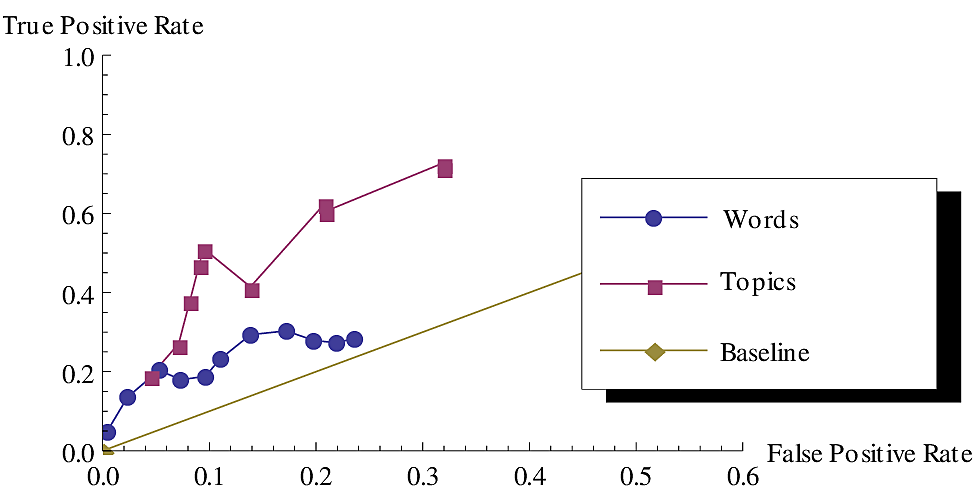
\includegraphics[width=0.48\linewidth]{figures/audio/campus/roc_top1_words_topics}
\label{fig:audio-roc-top1-campus}
}
\subfloat[]{
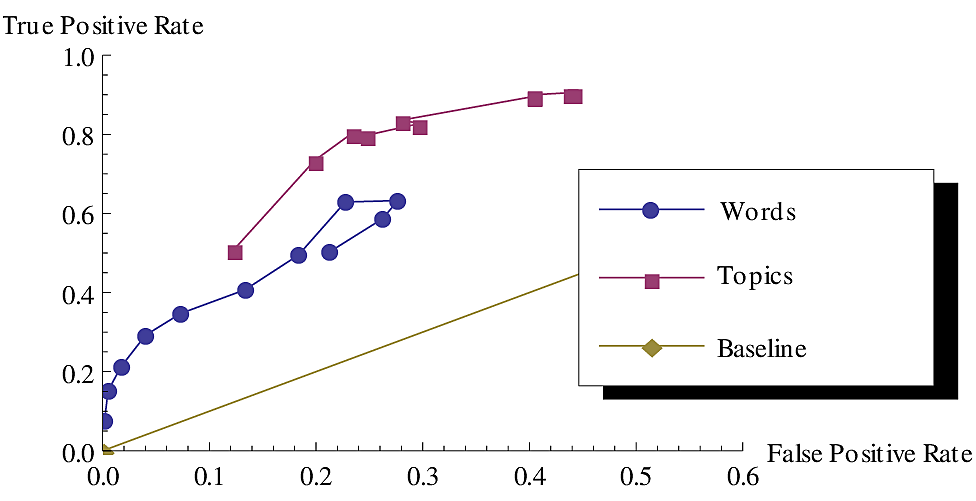
\includegraphics[width=0.48\linewidth]{figures/audio/figure8/roc_top1_words_topics}
\label{fig:audio-roc-top1-figure8}
}

\caption{ \emph{ROC curves for same-place recognition based on ambient sound:}
\protect\subref{fig:audio-roc-top1-campus} Four-loops dataset.
\protect\subref{fig:audio-roc-top1-figure8} Figure 8 dataset.
}
\label{fig:audio-roc-top1}
\end{center}
\end{figure}

Our experiments indicate that the temporal topic model finds a representation where a simple region assignment is much more meaningful than directly considering the features or using a topic model without any temporal considerations. Fixing the false positive rate to be less than 0.25, Table \ref{tab:audio-results-summary} shows the best detection accuracy for each algorithm for both the datasets. It should be noted that the reported false positive rate is probably higher than the actual false positive rate because similar sounding regions at physically different locations were marked as distinct in our ground truth. For example, regions (1) and (4) from the \emph{Figure-8} dataset are both recorded from busy streets, and sound the same, and as result are detected to be the same region by the proposed algorithm (Fig. \ref{fig:figure8-topicsg2}). From the similarity matrices produced by the system for the two datasets (Fig. \ref{fig:campus-topicsg4}, \ref{fig:figure8-topicsg2}), we can see that the algorithm is successfully able to detect loop closure at many, but not all locations.

In both datasets, the temporally smoothed topic-based region labels outperformed the top-word-based region labels. Further, the topic model with temporal independence of windows (the leftmost point in the topics line) does not significantly outperform the naive feature-based approach. This indicates how critical it is to explicitly model the dependencies between adjacent observations. To reiterate, we do not require topics to explicitly correspond to particular real-world regions. Yet in order to find a self-consistent region labelling where returning to the same location means our model will produce the same label we still must consider the temporal smoothness of region labels.

\begin{table}
    \centering
    \begin{tabular}{|c|c|c|c|c|c|c|}
    \hline
    Dataset & \multicolumn{6}{|c|}{Best Detection Accuracy}\\
    & \multicolumn{6}{|c|}{(False positive rate $<$ 0.25)}\\ \cline{2-7}
    &\multicolumn{2}{|c|}{MFCC-words}& \multicolumn{2}{|c|}{LDA}&\multicolumn{2}{|c|}{Temp. Smooth. LDA}\\
    \hline
    &TPR& FPR&TPR& FPR&~~ TPR ~~& FPR\\
    \hline
    Four-loops & 0.29 &0.15 & 0.19 & 0.04 & 0.61 & 0.21\\
    \hline
    Figure-8 & 0.63 & 0.23 & 0.50 & 0.12 & 0.80 & 0.23\\
    \hline
    \end{tabular}
    
    \caption{Best accuracy of unsupervised same place recognition from ambient sound.}
    \label{tab:audio-results-summary}
\end{table}

% \todo[inline]{really nice. bravo!}